\section{New industries, fads, and waves}\label{sec:waves}

This section asks when and where the leading penalty of
Section~\ref{sec:gate} lived: across registration cohorts, across the
technology classes, across the themes each era's leading filings were
drawn from, in the filings that name the internet, and inside surging
themes. The outcome throughout is the same one --- failure at the
five-year proof of continued use --- and every sample is settled cohorts
(registrations whose ninth anniversary is inside the record), so nothing
here is censored.

\subsection{The penalty weakened in the middle of the sample and was largest at the start}\label{sec:eras}

Scores exist from 1995, which makes registration cohorts from 1996
evaluable, and their outcomes at the five-year proof have been settled for
two decades. Figure~\ref{fig:cohortslopes} draws, for each cohort, the
change in survival for a one-standard-deviation increase in lead and in
atypicality, the two entered jointly and standardized within Nice class
and cohort. Pooled across classes, the lead coefficient is significantly
negative in every settled cohort except 2002--2005 --- $-1.9$ to $-2.3$pp
per standard deviation for the 1996--2000 cohorts, $+0.4$ to $-0.2$
across 2002--2005, and $-0.5$ to $-1.4$ from 2006 on. In the software
class the middle of the sample is not a pause but a reversal: the
coefficient runs from $-6.8$pp for the 1996 cohort to significantly
\emph{positive} ($+0.9$ to $+1.2$) in 2002, 2003 and 2005, then back
through $-4.0$ in 2012. The atypicality coefficient never changes sign
anywhere: more atypical registrations survive more in every cohort of
both panels, by $+0.6$ to $+2.5$pp per standard deviation pooled and
$+2.9$ to $+5.7$ in software.

\begin{figure}[h]\centering
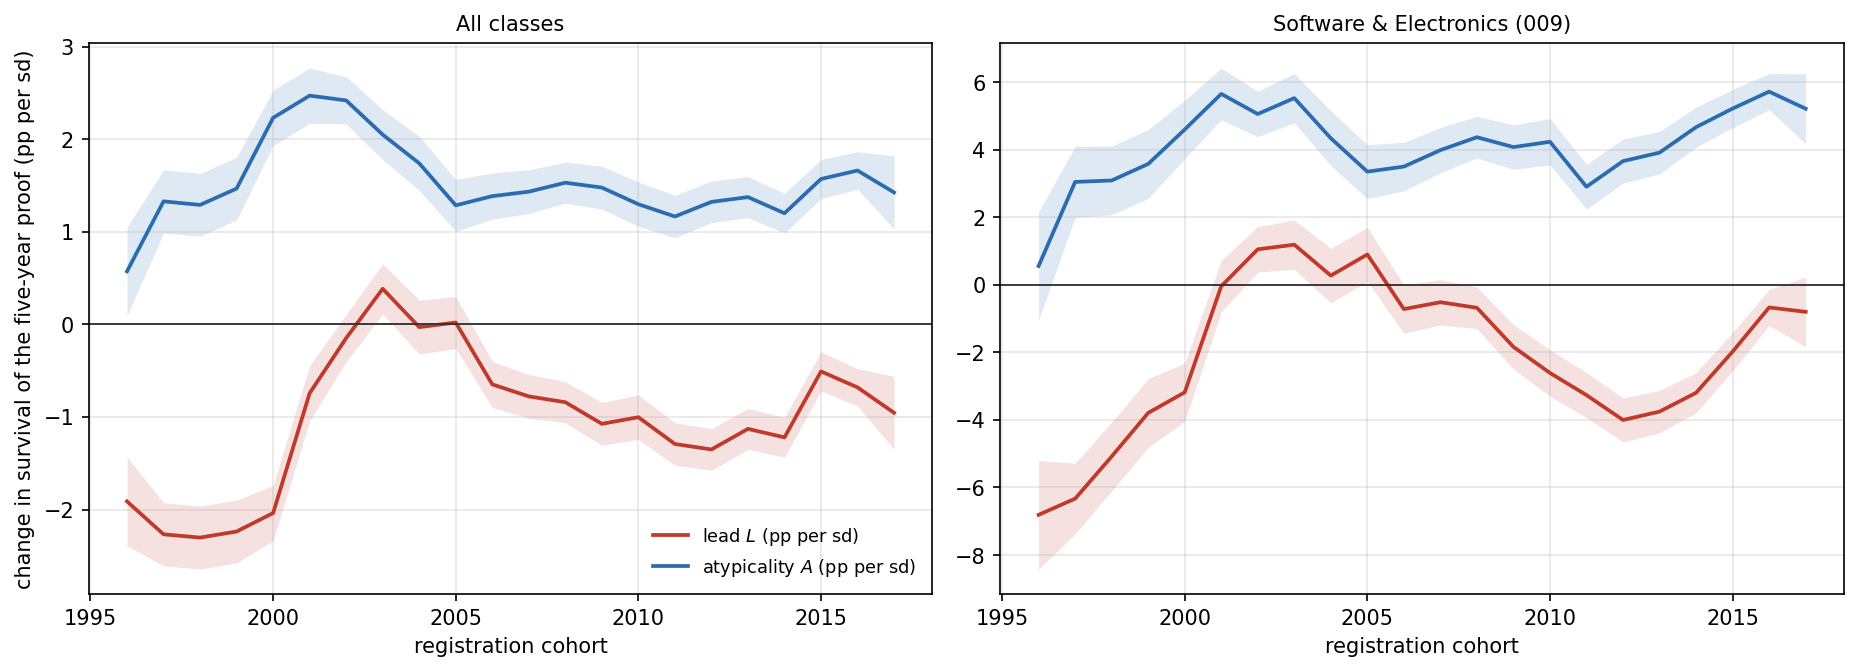
\includegraphics[width=\textwidth]{results/fig_cohort_slopes.png}
\caption{Survival of the five-year proof of continued use, per
registration cohort, as continuous coefficients: the change in survival,
in percentage points, for a one-standard-deviation increase in lead (red)
and in atypicality (blue), entered jointly, both standardized within Nice
class and cohort. Left: all classes pooled ($n = 3{,}150{,}442$ settled
registrations); right: software and electronics alone. Bands are 95\%
intervals on OLS standard errors, uncorrected for the within-owner
correlation of outcomes (0.38), so they understate the uncertainty
somewhat.}
\label{fig:cohortslopes}
\end{figure}

Stated as cohort contrasts, the swing is large: $+6.9$pp excess failure
for the most leading fifth in the 1996 cohort, rising to $+10.1$pp for
1999 --- roughly twice the largest cohort contrast observed since ---
then collapsing, and returning to $+1.8$ to $+5.6$pp for every cohort
from 2008. Scores begin in 1995, so a 1996-cohort registration must have
issued within a year of filing; early cohorts are selected on prosecution
speed. Holding pendency in a common one-to-three-year band leaves the
series unchanged. Indexing by filing year instead, so a cohort contains
every prosecution speed, gives $+7.9$ to $+9.6$pp for filings 1995--1999
and $-0.95$pp for filings made in 2000 --- a ten-point swing in a single
filing year.

Splitting the four classes that carry most technology filings --- 009,
035, 038 and 042 --- against the other forty-one separates a large moving
component from a small steady one (Figure~\ref{fig:eras}):

\begin{center}\small
\begin{tabular}{lrr}
\toprule
Filing years & Technology classes & All others \\
\midrule
1995--1999 & $+14.18$ (0.36) & $+4.48$ (0.27) \\
2000--2004 & $-1.37$ (0.35) & $+1.21$ (0.24) \\
2005--2007 & $+2.04$ (0.43) & $+1.99$ (0.28) \\
2008--2014 & $+9.02$ (0.25) & $+1.32$ (0.17) \\
\bottomrule
\end{tabular}
\end{center}

\noindent Outside technology the penalty is a flat $+1$ to $+4$pp in
every era, including the one in which the pooled series reads as zero.
Inside technology it swings by fifteen points: strongly positive for
filings made into the late 1990s, negative for those made in the five
years after, and positive again from 2008. The pooled quiet of 2002--2005
is a technology reversal partly offsetting a non-technology positive, not
an absence.

What this design cannot say is which cycle the swing belongs to. Marks
filed 1995--1999 reach their five-year proof in 2001--2007 and marks
filed 2000--2004 reach theirs in 2006--2013, so a story in which unusual
language is punished because it was written during an investment boom and
a story in which it is punished because the proof falls due during a bust
both fit these numbers.

\begin{figure}[h]\centering
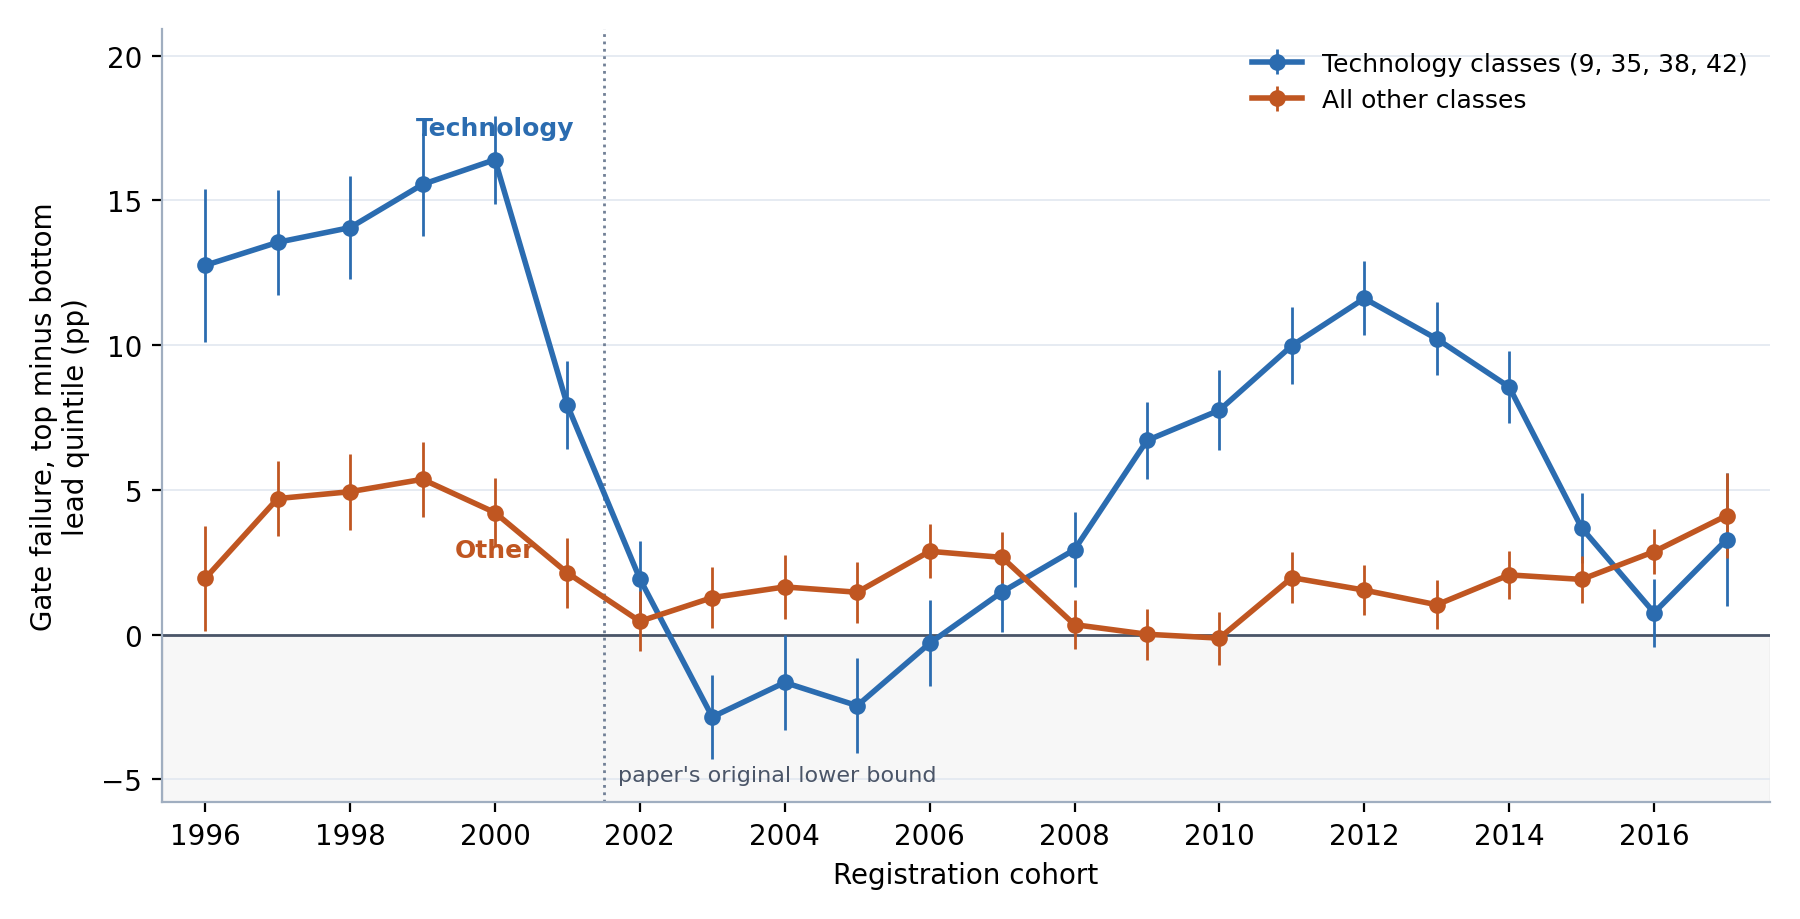
\includegraphics[width=0.86\textwidth]{results/gate_era_profile.png}
\caption{The leading penalty at the five-year proof by registration
cohort, technology classes (009, 035, 038, 042) against all others. Each
point is the failure rate of the most leading fifth of that cohort's
registrations minus that of the most lagging fifth, lead quintiles cut
within cohort and group, no controls, with 95\% intervals, on settled
registrations. Outside technology the penalty is small and almost flat
across two decades; inside technology it swings from $+16$pp for the 2000
cohort to $-3$pp for 2003 and back to $+12$pp for 2012. The dotted line
marks the 2002 cut that the cohort samples of Section~\ref{sec:gate}
use.}
\label{fig:eras}
\end{figure}

\subsection{Three of the four classes reverse, and the leading language changes theme}\label{sec:techswing}

The four-class split pools industries that do not move together. Taking
them one at a time, and then assigning quintiles inside progressively
finer cells (Table~\ref{tab:techswing}):

\begin{table}[h]\centering\small
\caption{The leading penalty at the five-year proof inside technology, by
class and by cell. Top-minus-bottom lead-quintile contrast in failure
(pp, SE in parentheses), settled registrations, by filing era. The upper
block assigns quintiles within each class and era. The lower block pools
the four classes and assigns quintiles within the era (raw), within
class$\times$registration-cohort cells, and within
theme$\times$class$\times$registration-year cells, where a filing's theme
is the one its description loads most heavily on under the production
$T = 50$ model. $n = 1{,}248{,}591$.}
\label{tab:techswing}
\begin{tabular}{lrrrr}
\toprule
Class & 1995-1999 & 2000-2004 & 2005-2007 & 2008-2014 \\
\midrule
009 Electrical, software & $+18.04$ (0.52) & $-5.32$ (0.51) & $+0.25$ (0.62) & $+11.67$ (0.37) \\
035 Business services & $+4.59$ (0.69) & $-9.70$ (0.56) & $+2.02$ (0.63) & $+1.66$ (0.36) \\
038 Telecommunications & $+9.91$ (1.40) & $-4.24$ (1.29) & $+2.60$ (1.48) & $+3.42$ (0.94) \\
042 Scientific, computer services & $+17.11$ (0.57) & $+6.70$ (0.62) & $+8.42$ (0.87) & $+12.63$ (0.47) \\
\midrule
Four classes pooled, raw & $+14.49$ (0.33) & $-1.81$ (0.31) & $+2.56$ (0.38) & $+9.16$ (0.22) \\
\quad within class$\times$cohort & $+14.27$ (0.33) & $-3.63$ (0.31) & $+2.73$ (0.38) & $+7.24$ (0.22) \\
\quad within theme$\times$class$\times$cohort & $+4.78$ (0.33) & $-1.26$ (0.31) & $+2.56$ (0.38) & $+4.51$ (0.22) \\
\bottomrule
\end{tabular}

\end{table}

\noindent Electrical and software goods (009) and telecommunications
(038) follow the pooled pattern. Business services (035), the class that
holds online retail, reverses hardest: $-9.7$pp for filings made
2000--2004 against $+4.6$pp in the five years before. Scientific and
computer services (042) never reverses. Its contrast is $+6.7$pp in the
era in which the other three are negative and between $+8$ and $+17$pp in
every other, and by registration cohort it never falls below $+3$pp
(Figure~\ref{fig:techswing}). The reversal is an event in goods and in
business services; the class that sells technology as a service sat it
out.

Assigning quintiles within class and registration year rather than within
the era pool changes little. Assigning them within theme, class and
registration year changes a great deal: the late-1990s contrast falls
from $+14.5$ to $+4.8$pp, the post-2008 contrast from $+9.2$ to $+4.5$pp,
and the 2000--2004 reversal from $-3.6$ to $-1.3$pp. Two thirds of the
first and half of the second are between themes rather than within them.
The leading fifth of each era was drawn from particular themes, and those
themes carried their own failure rates; the penalty for being leading
\emph{inside} a theme is a steadier $+2.5$ to $+5$pp, the same order as
the penalty outside technology.

Which themes is a matter of record (Table~\ref{tab:techthemes}; the
table's last row is the all-themes pooled contrast within
theme$\times$class$\times$cohort). In 1995--1999 the computer, software,
information and data services theme held 38\% of technology filings and
75\% of the leading fifth, and its registrations from those filing years
failed at 64.9\% against 47.5--59.0\% in the other large themes. That one
theme is most of the late-1990s penalty. In 2000--2004 it held 12\% of
the leading fifth. The leading language had moved to video, music and
games on electronic media (31\% of the leading fifth against 12\% of
filings) and the internet-services language had become lagging ---
wording the class was leaving --- and inside several themes the lagging
fifth now failed more than the leading one: $-3.6$pp in electronic media,
$-5.5$ in retail store services, $-6.9$ in apparatus and control systems.
From 2008 the leading fifth over-represents downloadable and online
software by four to one (15\% against 4\%), the vocabulary of the
application store; those registrations fail at 67.2\% over the whole
period, the highest base rate of any theme, and their within-theme lead
contrast pooled across cohorts, $+8.4$pp, is the largest of any theme
(the table's 2008--2014 cell, cut within that era alone, is $+3.3$pp).
The computer-services theme's own contrast is positive in every era
($+3.6$ to $+5.9$pp) and never reverses.

\begin{table}[h]\centering\footnotesize
\caption{The leading penalty at the five-year proof by theme within the
four technology classes. Themes with at least 20{,}000 settled
registrations, labelled by their five highest-probability terms;
quintiles assigned within theme and era. Cells with fewer than 3{,}000
registrations are blank. The final row pools all themes, with quintiles
cut within theme$\times$class$\times$cohort.}
\label{tab:techthemes}
\begin{tabular}{p{5.2cm}rrrrr}
\toprule
Theme (top words) & $n$ & 1995-1999 & 2000-2004 & 2005-2007 & 2008-2014 \\
\midrule
services, computer, software, information, data & 451,253 & $+3.61$ (0.52) & $+3.56$ (0.49) & $+4.18$ (0.64) & $+5.92$ (0.37) \\
video, computer, electronic, music, games & 162,290 & $+2.53$ (0.97) & $-3.62$ (0.89) & $-2.85$ (1.01) & $+3.36$ (0.60) \\
services, featuring, store, retail, store services & 131,107 & $+8.39$ (1.09) & $-5.49$ (1.01) & $+2.92$ (1.15) & $+0.98$ (0.66) \\
services, field, training, estate, educational & 95,602 & $+7.82$ (1.09) & $+0.99$ (1.12) & $+6.02$ (1.43) & $+2.05$ (0.83) \\
apparatus, systems, devices, electronic, control & 84,121 & $+4.80$ (1.27) & $-6.92$ (1.19) & $-0.58$ (1.41) & $+3.65$ (0.88) \\
design, field, systems, development, services & 32,517 & $+10.40$ (2.03) & $+4.67$ (1.82) & $+1.50$ (2.27) & $-2.27$ (1.45) \\
software, online, downloadable, non-downloadable, virtual & 29,472 & --- & --- & --- & $+3.30$ (1.05) \\
bags, clothing, shirts, jackets, leather & 28,421 & $+1.28$ (2.59) & $-1.55$ (2.39) & $-4.66$ (2.40) & $+6.06$ (1.36) \\
research, medical, scientific, testing, purposes & 25,897 & $+12.65$ (2.66) & $+12.09$ (2.03) & $-3.82$ (2.59) & $+5.63$ (1.51) \\
services, health, field, care, information & 22,880 & $+4.94$ (2.04) & $+1.39$ (2.36) & --- & $+3.50$ (1.72) \\
\midrule
All themes, within theme$\times$class$\times$cohort & 1,150,921 & $+4.78$ (0.33) & $-1.26$ (0.31) & $+2.56$ (0.38) & $+4.51$ (0.22) \\
\bottomrule
\end{tabular}

\end{table}

\begin{figure}[h]\centering
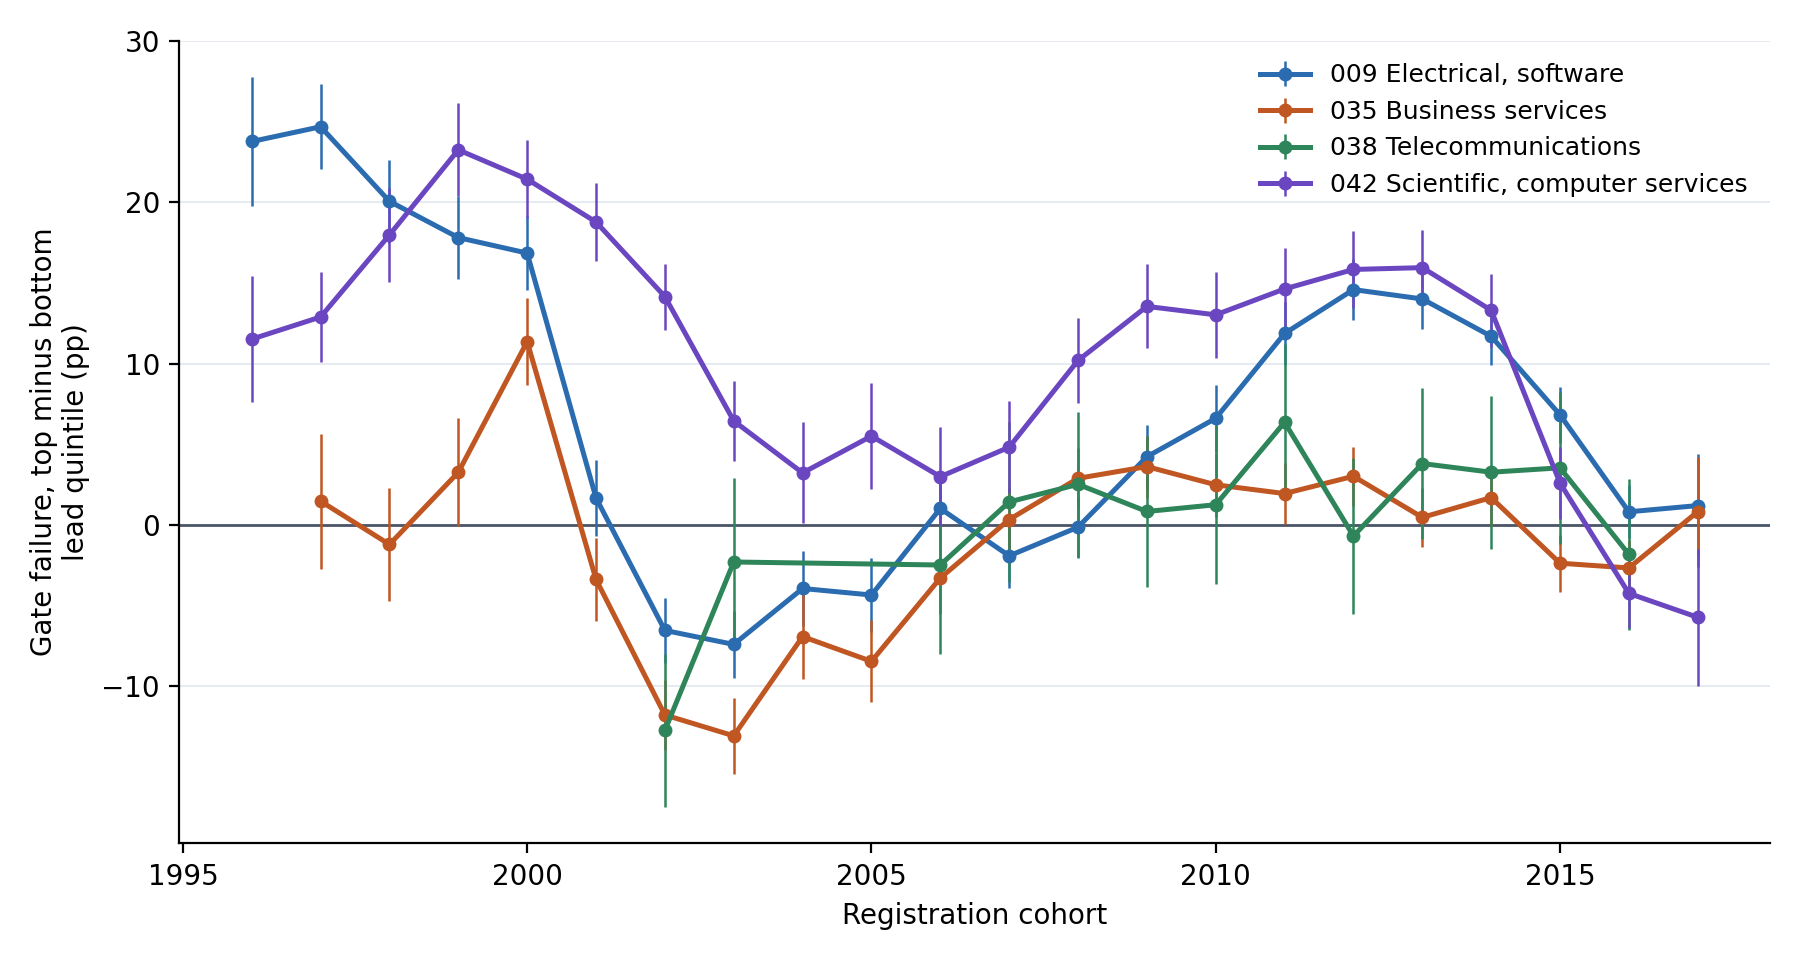
\includegraphics[width=0.92\textwidth]{results/gate_era_tech_themes.png}
\caption{The leading penalty at the five-year proof by registration
cohort, one line per technology class. Each point is the failure rate of
the most leading fifth of that class and cohort's registrations minus
that of the most lagging fifth --- lead quintiles cut within class and
cohort, no controls --- with 95\% intervals, on settled registrations.
Three classes cross zero between 2001 and 2006; scientific and computer
services does not.}
\label{fig:techswing}
\end{figure}

So the swing has two layers. Across the whole period, a leading filing is
a few points more likely to fail than a lagging one in the same theme,
class and cohort, in technology as elsewhere. On top of that, each era's
leading vocabulary was concentrated in one or two themes whose marks
failed at their own rate: internet services in the 1990s, application
software after 2008. In the trough between, the language that had been
leading became lagging, and the marks still written in it failed with it.
The design-based estimates of Table~\ref{tab:gate_lpm} hold class and
cohort fixed but not theme, so they carry both layers; a reader who wants
only the within-theme penalty should take the lower block of
Table~\ref{tab:techswing} as the guide to its size.

\subsection{Internet as a theme: web-based filings against their class}\label{sec:internet}

A filing is internet-bearing when its goods/services text names the
internet, the web, a website, online or on-line provision, or electronic
commerce. The rule reads the text rather than the class, so a web
retailer filing in apparel is caught and a semiconductor maker filing in
class 009 is not. Internet-bearing filings are 16.9\% of scored
registrations: 58\% in telecommunications, 39--41\% in advertising and
retail, scientific and technical services, and legal and personal
services, under 5\% in most goods classes.
Figure~\ref{fig:webscatter} puts every class on two axes at once --- how
much more often its internet-bearing filings register, and how much more
often they fail the five-year proof --- and
Table~\ref{tab:internet} carries the underlying rates.

\begin{figure}[h]\centering
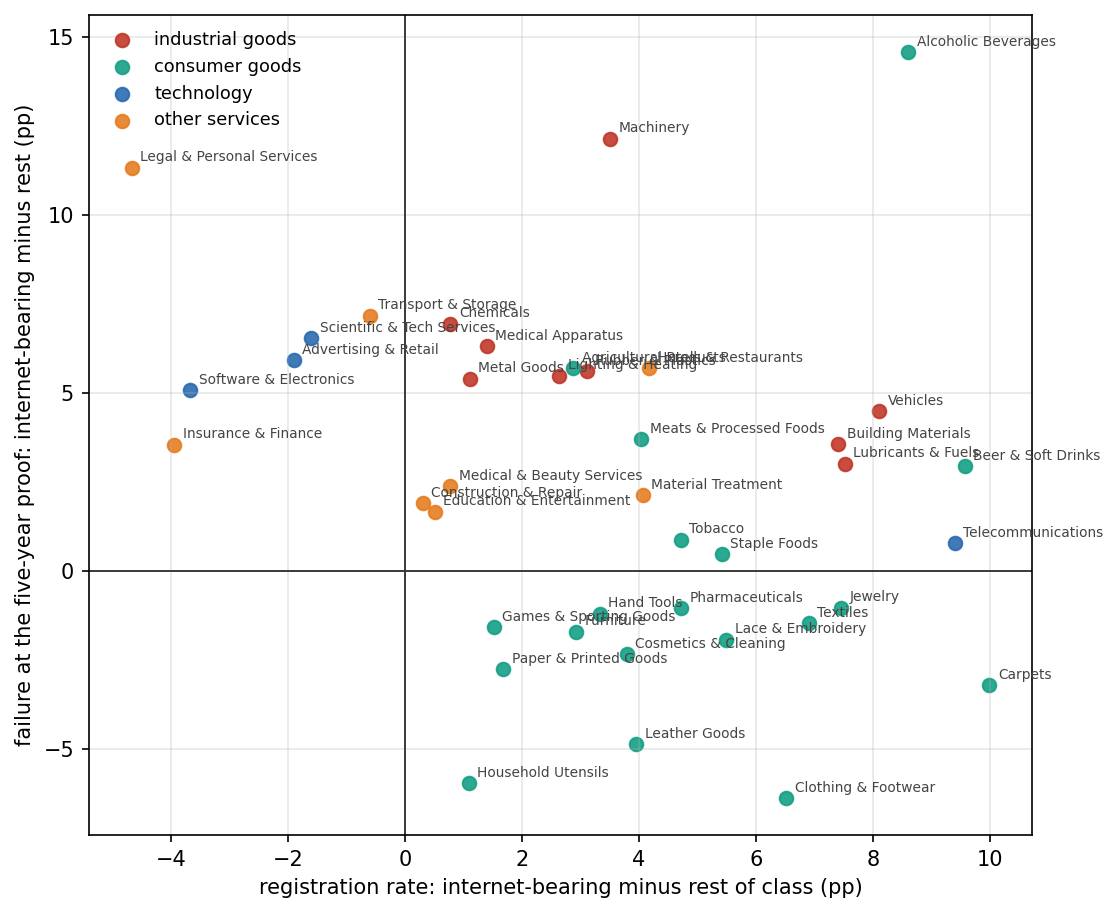
\includegraphics[width=0.8\textwidth]{results/fig_internet_scatter.png}
\caption{Each Nice class's internet-bearing filings against the rest of
the class, on both steps at once. Horizontal: registration rate of
internet-bearing class-records minus the rest of the class, filings
1995--2018. Vertical: failure at the five-year proof of continued use,
internet-bearing minus the rest, registrations 2002--2018. Classes with
fewer than 500 internet-bearing registrations are dropped. Classes in the
upper-right quadrant grant internet filings more often and lose them
more often.}
\label{fig:webscatter}
\end{figure}

\begin{table}[h]\centering\footnotesize
\caption{Internet-bearing filings against the rest of their Nice class.
Registration is the share of class-records filed 1995--2018 that reached
registration; failure is the share of unique registrations 2002--2018
cancelled for non-use at age 4.0--8.5 years. Classes with fewer than 500
internet-bearing registrations are omitted.}
\label{tab:internet}
\begin{tabular}{llrrrrr}
\toprule
Class & & Web share & \multicolumn{2}{c}{Registration (\%)} & \multicolumn{2}{c}{Gate failure (\%)} \\
 & & (\%) & web & rest & web & rest \\
\midrule
001 & Chemicals & 1.8 & 65.0 & 64.3 & 46.1 & 39.1 \\
003 & Cosmetics \& Cleaning & 2.8 & 58.0 & 54.2 & 52.1 & 54.4 \\
004 & Lubricants \& Fuels & 4.6 & 63.8 & 56.3 & 50.9 & 47.9 \\
005 & Pharmaceuticals & 1.9 & 53.3 & 48.6 & 52.4 & 53.5 \\
006 & Metal Goods & 3.5 & 68.1 & 67.0 & 44.5 & 39.1 \\
007 & Machinery & 2.8 & 73.3 & 69.7 & 50.9 & 38.7 \\
008 & Hand Tools & 3.6 & 65.8 & 62.5 & 42.4 & 43.6 \\
009 & Software \& Electronics & 18.7 & 53.3 & 57.0 & 56.5 & 51.4 \\
010 & Medical Apparatus & 3.0 & 59.8 & 58.4 & 51.7 & 45.4 \\
011 & Lighting \& Heating & 3.0 & 67.4 & 64.8 & 51.4 & 45.9 \\
012 & Vehicles & 3.4 & 69.0 & 60.9 & 49.6 & 45.1 \\
014 & Jewelry & 7.4 & 63.2 & 55.8 & 54.7 & 55.7 \\
016 & Paper \& Printed Goods & 15.1 & 57.8 & 56.1 & 47.9 & 50.7 \\
017 & Rubber \& Plastics & 2.2 & 70.7 & 67.6 & 44.1 & 38.5 \\
018 & Leather Goods & 8.0 & 61.4 & 57.4 & 50.5 & 55.4 \\
019 & Building Materials & 2.0 & 71.4 & 64.0 & 47.5 & 43.9 \\
020 & Furniture & 4.2 & 62.2 & 59.2 & 47.0 & 48.7 \\
021 & Household Utensils & 5.1 & 60.1 & 59.0 & 44.5 & 50.5 \\
024 & Textiles & 6.0 & 62.8 & 55.9 & 49.7 & 51.2 \\
025 & Clothing \& Footwear & 5.6 & 56.1 & 49.6 & 52.4 & 58.7 \\
026 & Lace \& Embroidery & 7.6 & 61.2 & 55.7 & 52.0 & 53.9 \\
027 & Carpets & 5.6 & 66.8 & 56.8 & 43.7 & 46.9 \\
028 & Games \& Sporting Goods & 6.3 & 55.1 & 53.6 & 54.1 & 55.7 \\
029 & Meats \& Processed Foods & 2.5 & 59.7 & 55.7 & 53.3 & 49.6 \\
030 & Staple Foods & 2.6 & 61.4 & 56.0 & 52.3 & 51.8 \\
031 & Agricultural Products & 2.5 & 60.9 & 58.0 & 49.5 & 43.8 \\
032 & Beer \& Soft Drinks & 2.4 & 58.7 & 49.1 & 56.2 & 53.3 \\
033 & Alcoholic Beverages & 1.2 & 61.3 & 52.7 & 56.9 & 42.3 \\
034 & Tobacco & 2.9 & 53.8 & 49.1 & 55.0 & 54.2 \\
035 & Advertising \& Retail & 40.7 & 59.3 & 61.2 & 57.9 & 52.0 \\
036 & Insurance \& Finance & 18.9 & 58.6 & 62.6 & 52.4 & 48.9 \\
037 & Construction \& Repair & 10.4 & 67.8 & 67.5 & 49.0 & 47.1 \\
038 & Telecommunications & 57.6 & 54.5 & 45.1 & 60.8 & 60.1 \\
039 & Transport \& Storage & 21.3 & 62.5 & 63.1 & 54.8 & 47.6 \\
040 & Material Treatment & 9.6 & 68.0 & 63.9 & 49.4 & 47.3 \\
041 & Education \& Entertainment & 35.0 & 61.1 & 60.6 & 54.2 & 52.5 \\
042 & Scientific \& Tech Services & 39.3 & 57.8 & 59.4 & 58.0 & 51.4 \\
043 & Hotels \& Restaurants & 9.1 & 62.9 & 58.7 & 53.8 & 48.1 \\
044 & Medical \& Beauty Services & 20.6 & 62.9 & 62.1 & 53.7 & 51.3 \\
045 & Legal \& Personal Services & 41.5 & 60.3 & 65.0 & 60.1 & 48.7 \\
\bottomrule
\end{tabular}

\end{table}

Three patterns are in the figure. In the industrial goods classes,
internet-bearing registrations fail the five-year proof far more often
than their class: machinery 50.9\% against 38.7\%, chemicals 46.1\%
against 39.1\%, vehicles 49.6\% against 45.1\%. A web-based business
registering in an engineering class fails at the rate of a software
registration (51.4\%), not at the rate of its class. In the consumer
goods classes the sign reverses --- internet-bearing registrations in
clothing fail 52.4\% against 58.7\% for the class, in household utensils
44.5\% against 50.5\% --- so online sellers of consumer goods outlast the
class's other registrants. In every service class the internet-bearing
filings fail more often, by one to eleven points, most in legal and
personal services (60.1\% against 48.7\%). At the registration step the
industrial-goods classes sit to the right of zero: internet-bearing
applications there reach registration 59.5\% of the time against 56.0\%
for the rest. For those classes the two steps move in opposite
directions --- more likely to be granted, then more likely to be
cancelled for non-use six years later --- which is the pattern
Section~\ref{sec:gate_conclusion} predicts when the examiner reads
distance from class language and the market reads whether the product
stayed in commerce.

The failure gap has a common shape in event time. Dating the internet's
arrival in each class as the first filing year in which the pattern
reaches 2\% of the class's filings (1994--1995 in the technology and
transport classes, 1999--2000 in apparel and chemicals, 2008 in
machinery), and aligning each class's per-cohort gap on years since its
own arrival: the gap starts near $+7$ points in the first observable
cohorts, declines to about zero nine to eleven years after arrival, and
settles between $+1$ and $+4$ (Figure~\ref{fig:webshape}). Across the
eight classes observable in both phases, the mean gap is $+4.4$ points in
years zero to four and $+1.6$ from year ten, shrinking in six of the
eight. Calendar time disguises this: transport, whose arrival was 1995,
peaks at $+16$ points in its 2000 cohort and declines; machinery, whose
arrival was 2008, peaks at $+17$ points in its 2012--2015 cohorts --- its
own early years. The class's clock starts when the vocabulary arrives,
not when the internet did. Clothing is the standing exception: its
internet-bearing registrations outlast the class in every cohort after
2004, consistent with online sellers of goods surviving where early
web-services ventures did not.

One reading of the early-cohort excess is entry cost. Opening a web-based
business in a class's first internet years required little capital and
little prior experience in the trade, while capital for exactly such
ventures was abundant; a step that filters on whether a product held its
place in commerce for five years will fail cheap entries at a higher
rate wherever they cluster, and they clustered in each class's first
internet cohorts. The record cannot test founders' costs directly, but
the event-time shape --- highest at each class's own arrival, fading as
the channel became ordinary --- is what falling entry barriers followed
by normalization would leave.

\begin{figure}[h]\centering
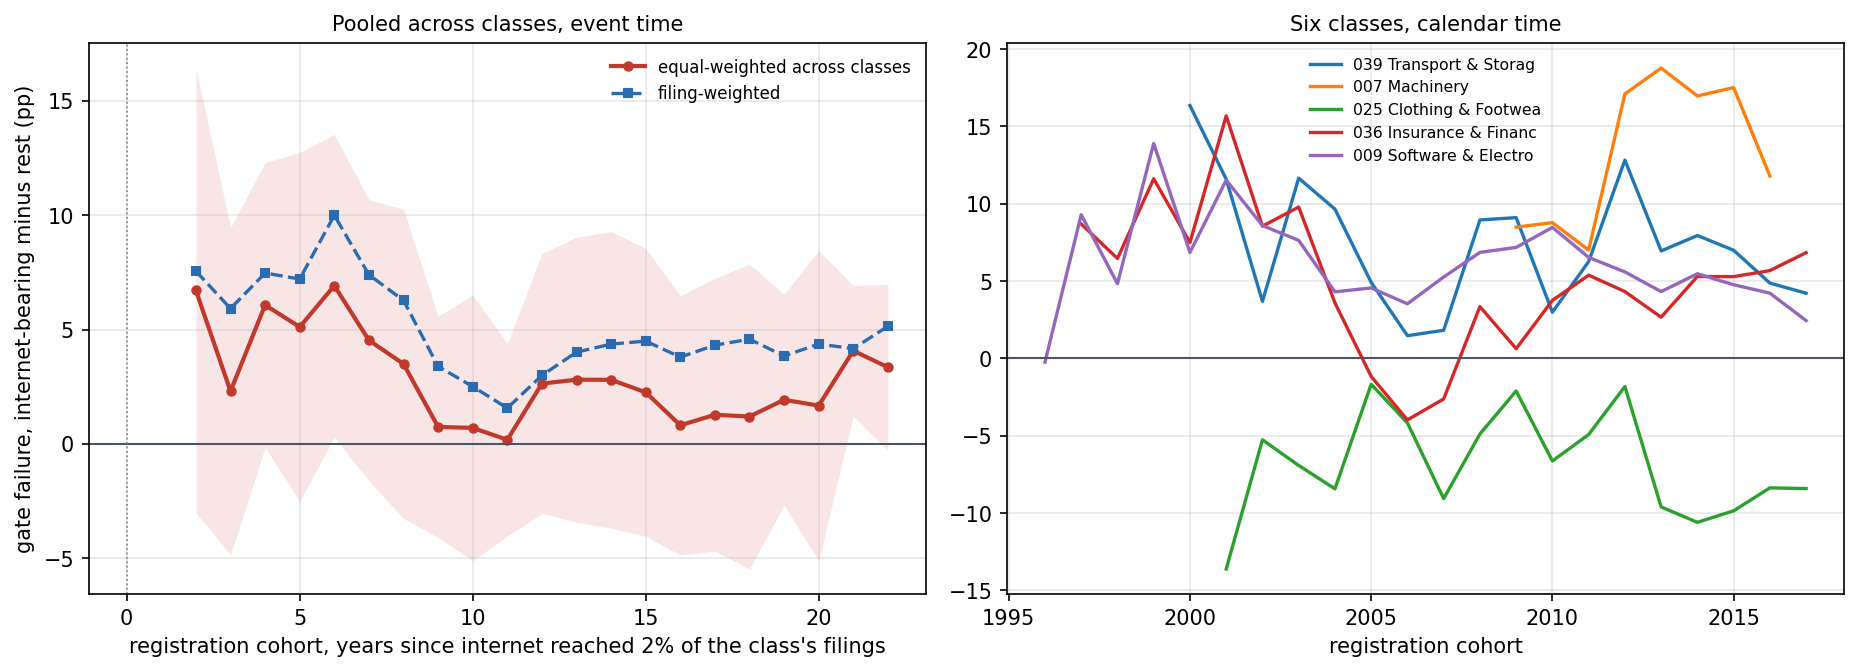
\includegraphics[width=\textwidth]{results/internet_convergence.png}
\caption{The internet gap in failure at the five-year proof, inside each
class. \emph{Left:} internet-bearing minus other registrations' failure
rate, by registration cohort in years since the internet pattern reached
2\% of the class's filings, averaged across classes (band: one standard
deviation across classes). \emph{Right:} five classes in calendar time.
Cells with fewer than 100 registrations in either group are dropped.}
\label{fig:webshape}
\end{figure}

The internet split also locates the era swing of
Section~\ref{sec:eras}. Rerunning the per-cohort lead coefficients of
Figure~\ref{fig:cohortslopes} separately for internet-bearing and other
registrations (Figure~\ref{fig:webslopes}): the mid-sample reversal
belongs to the internet-bearing filings, whose leading registrations
survived \emph{more} in the 2001--2005 cohorts ($+1.3$ to $+2.5$pp per
standard deviation) while non-internet technology registrations sat near
zero. The other two episodes are not the internet's in this textual
sense. The late-1990s penalty is present in technology registrations that
never name the web ($-3.4$ to $-4.8$pp for the 1996--2000 cohorts) ---
consistent with Table~\ref{tab:techthemes}, where that era's deadly
vocabulary is computer and software services, words that predate explicit
internet naming. And the post-2008 penalty sits in both splits at once
($-2$ to $-3$pp each). Outside technology, the non-internet series is
the steady $-0.4$ to $-1.4$pp throughout. What the internet changed, on
this cut, is the middle: for half a decade after the crash, the web
filings whose language led their class were the ones that lasted.

\begin{figure}[h]\centering
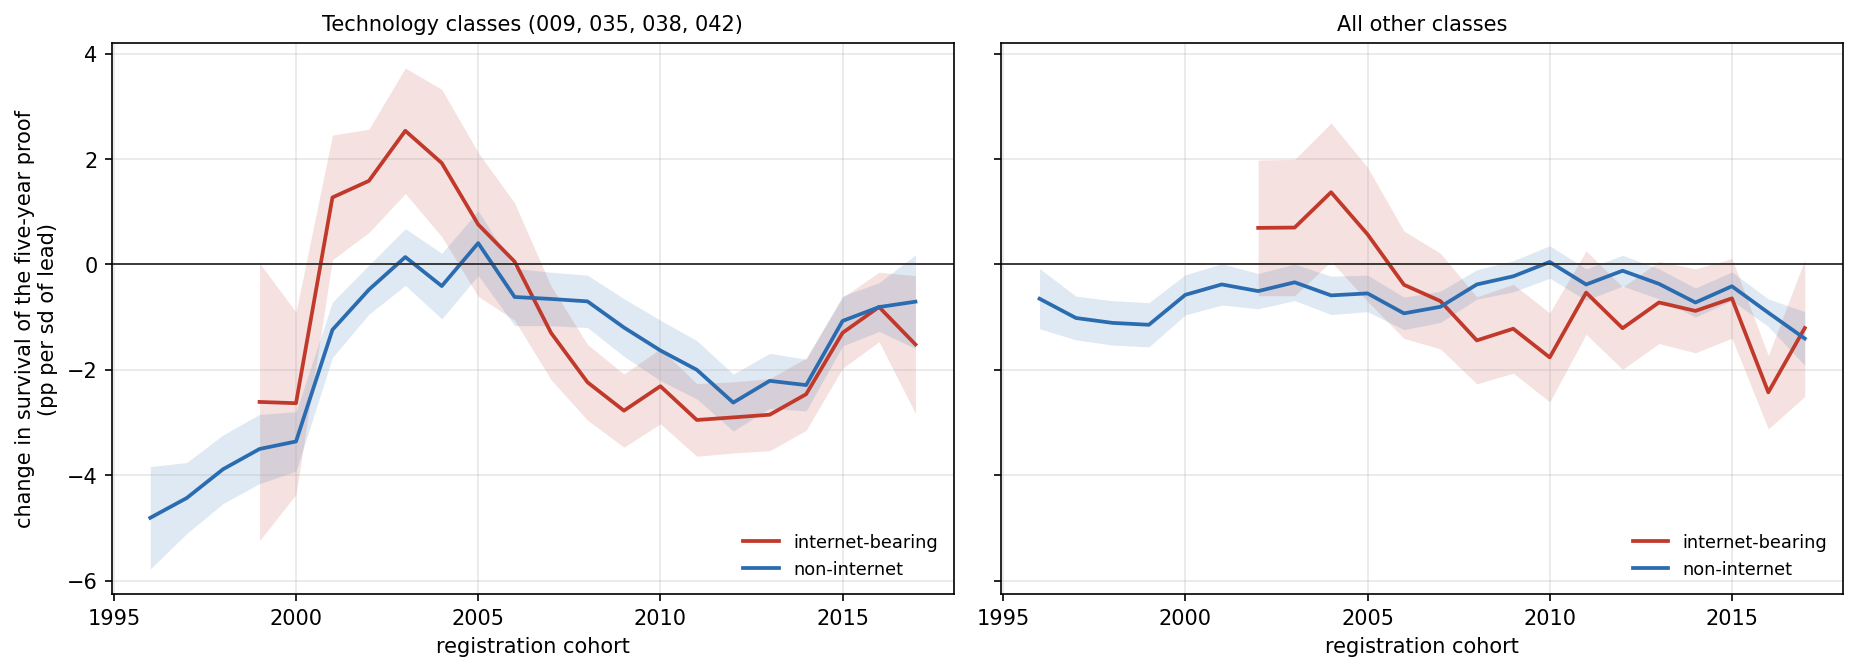
\includegraphics[width=\textwidth]{results/fig_cohort_slopes_internet.png}
\caption{The per-cohort lead coefficient of Figure~\ref{fig:cohortslopes},
split by the curated internet text pattern: change in survival of the
five-year proof per standard deviation of lead, atypicality held,
standardized within Nice class and cohort. Left: the four technology
classes; right: all other classes. Bands are 95\% intervals on OLS
standard errors; cohort cells under 2{,}000 registrations are dropped,
which is why the internet-bearing lines start late.}
\label{fig:webslopes}
\end{figure}

The classification system has faced this question and twice declined to
make the internet a class. Before 2002, internet and computer services
accumulated in class 42, whose heading then ended ``services that cannot
be classified in other classes''; the Nice Union's Committee of Experts
restructured it in the eighth edition, effective 1 January 2002, by
narrowing 42 to scientific and technological services and moving the rest
into three new classes (43--45), organised by the kind of service rather
than by the technology.\footnote{Nice Classification, 8th edition (WIPO,
2002); the USPTO's guidance describes the class-42 restructuring. The
eighth edition took effect in the middle of the era swing of
Section~\ref{sec:eras}.} The question returned with virtual goods: the
twelfth edition, effective 1 January 2023, classifies downloadable
virtual goods and NFT-authenticated files in class 9 and distributes
metaverse-related services across the existing service classes, again
declining a new class.\footnote{Nice Classification, 12th edition (WIPO,
2023).} The pattern above bears on that choice. Internet-bearing filings
in a goods class survive or fail at rates closer to the technology
classes than to their own class, so for the outcome this paper measures,
the technology overlay carries more information than the class assignment
it is filed under. A classification built for scope of protection has no
reason to track survival; but a reader using Nice classes as industry
controls, as this paper and the literature do, should know that the
internet cuts across them.

\subsection{Surges: joining a wave}\label{sec:surge}

Genuinely new themes are rare (Section~\ref{sec:three_scorings}); the
observable event is a surge, an established theme's share doubling, over
its own three prior years, to a level that matters.
Figure~\ref{fig:surges} draws four episodes: their share trajectories,
and how their registrations fared at the five-year proof.

\begin{figure}[h]\centering
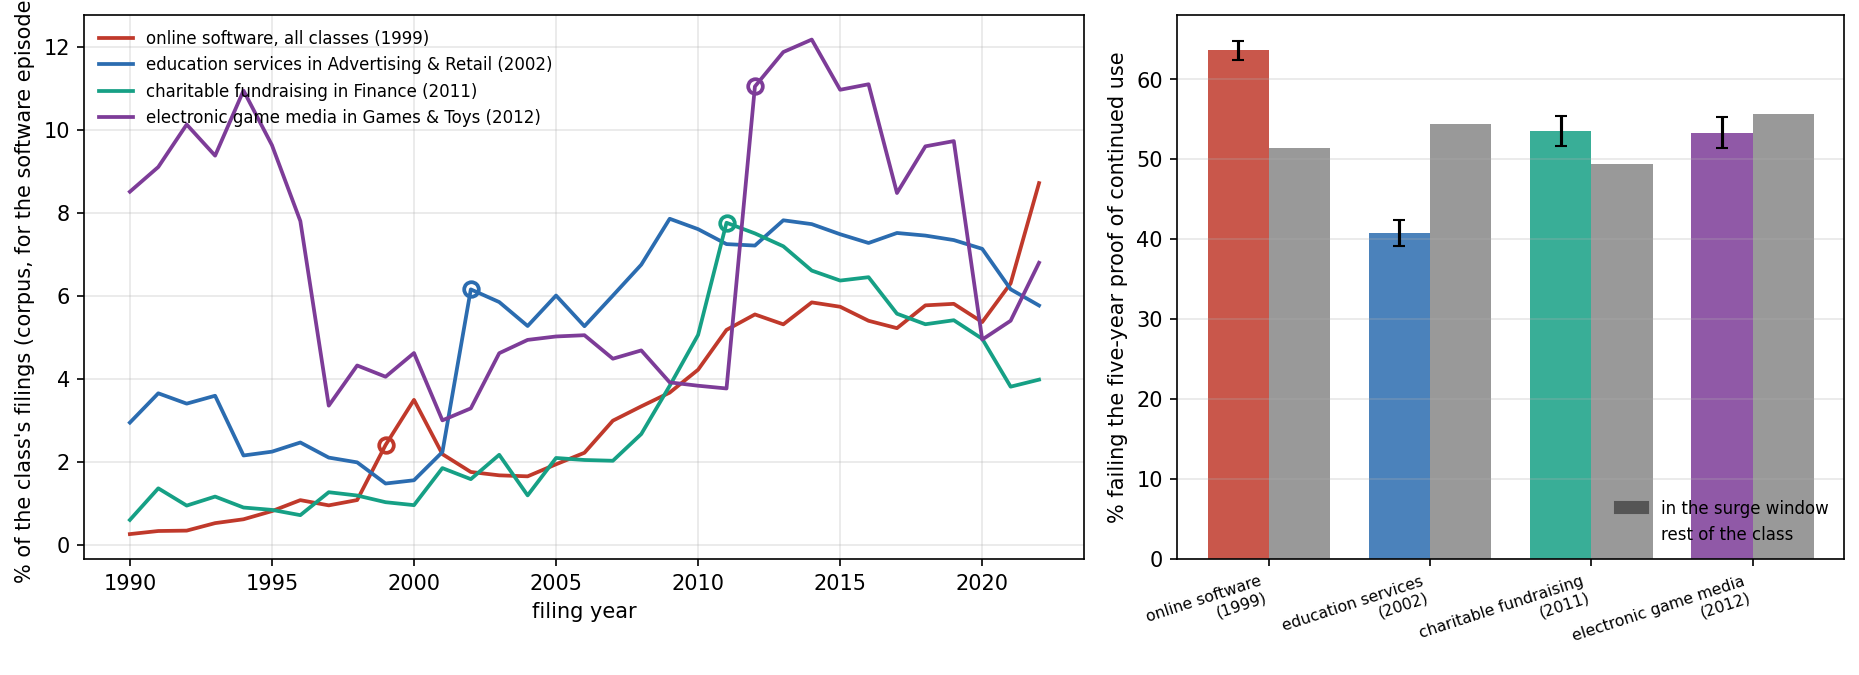
\includegraphics[width=\textwidth]{results/fig_surges.png}
\caption{Four surge episodes under the 500-theme model. \emph{Left:} the
theme's share of its class's filings by filing year (for the online
software episode, of all filings corpus-wide), on the 25\% systematic
sample the surge screen uses; the open circle marks the surge year, the
first in which the share doubled its own three-year prior mean above the
threshold. \emph{Right:} failure at the five-year proof of continued use
for registrations whose dominant theme was the surging one, filed in the
three-year surge window (colored, 95\% intervals), against the rest of
the same class in the same cohorts (grey).}
\label{fig:surges}
\end{figure}

Measured against the whole corpus at a 1\% share, five themes ever surge,
and one episode clears a 1{,}000-registration floor: the
online-and-downloadable-software theme doubled to 2.4\% of all filings in
1999. The 6{,}339 registrations whose dominant theme it was during
1999--2001 failed the five-year proof at 63.7\%, $8.6$ points above their
class and year and $8.5$ net of their own lead and atypicality. Within
the episode, the most leading fifth failed no more than the most lagging
($-0.2$pp, SE $1.9$).

Measured within a class at the same thresholds, surges are common: 962
episodes of a theme doubling to at least 1\% of its class, holding
32{,}418 registrations at the five-year proof. Pooled, being in one of
these smaller waves costs little: in-surge registrations fail $0.65$
points more than their class and year, $1.27$ net of lead and atypicality
($1.33$ and $1.70$ at the 2\% threshold). The episodes differ in sign
among themselves, as the figure's right panel shows: the
education-services surge in advertising and retail after 2002 failed
$13.7$ points less than its class; the charitable-fundraising surge in
finance after 2011 failed $4.0$ points more. Of the few episodes large
enough to carry their own lead contrast, one is clearly positive (the
education-services surge, $+5.8$pp, $t = 2.2$) and the rest are
indistinguishable from zero.

Three further facts about the waves, on the 61 episodes with at least 300
joining registrations over a six-year entry window --- 64{,}105 of the
86{,}447 registrations that join any episode. First, within a wave, entry
order does not matter: demeaned within episode, joiners in the surge year
fail $-0.8$ points relative to their wave's mean, joiners five years in
$+0.0$, with no gradient between (each SE about $0.5$). Second, among
class-scale waves, larger is not deadlier: excess failure is $+2.7$
points in the smallest tercile of waves, $+3.9$ in the middle, $-0.1$ in
the largest, and correlates with wave size at $-0.22$. The eight-point
excess of the corpus-scale software wave is not the top of a
dose-response within classes; it is a different scale of event. Third,
call a wave growing when the theme's share five years after the surge is
at or above its surge level. Growing waves carry more excess failure
($+4.3$ points, 22 episodes) than receding ones ($+1.0$, 39 episodes).
That runs against reading the excess as pure fad mortality, in which the
collapsing waves should be the deadly ones, and against under-response,
in which joiners of durable waves should thrive. A reading consistent
with all three facts is selection at the proof rather than crowding out:
a surging theme draws registrations for products that were never brought
to use at higher rates wherever the theme is commercially active, and the
theme's own subsequent growth does not rescue them. With 22 growing
episodes whose individual excesses range from $-13.7$ to $+4.0$ points,
the $3.3$-point difference between growing and receding waves is
suggestive, not settled.

\subsection{What the waves show}\label{sec:waves_conclusion}

The leading penalty is steady and small outside technology and episodic
inside it, and most of the episode is between themes: each era's leading
vocabulary was concentrated in one or two themes that failed at their own
rate, while the within-theme penalty holds at $+2.5$ to $+5$pp
throughout. Web-based filings fail hardest in each class's own first
internet years and converge toward their class within a decade. Joining a
surging theme costs little on average and nothing for arriving early
within the wave; the one corpus-scale wave, online software in 1999, is
the exception at every margin. What a fad costs, on this record, is
mostly a matter of which theme the fad was, not of when the filer joined
it.
